\subsection{Краевые состояния}
Несмотря на то, что у топологического изолятора есть щель в объёмном спектре,
на его границе возникают киральные
краевые состояния, пересекающие щель.  
Состояния с различными спинами образуют крамерсовский дублет и
движутся в противоположных направлениях. Поэтому никакое T--инвариантное возмущение не может
привести к их рассеянию друг в друга, см. приложение~\ref{app:kramers_doublet}. 
При отсутствии рассеяния край топологического изолятора
ведёт себя как идеальный провод: состояния не будут локализованы.

\begin{figure}[h]
    \centering
    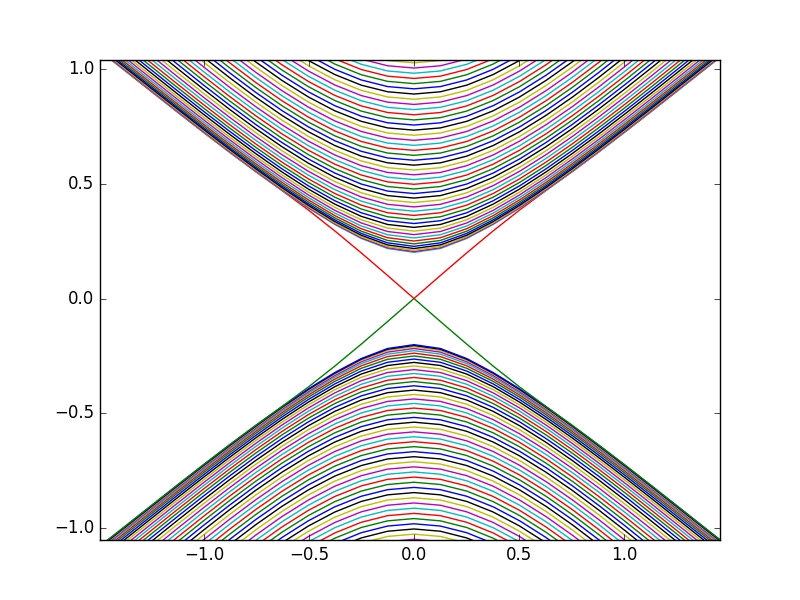
\includegraphics[width=0.6\linewidth]{edge_states.png}
    \caption{Спектр полосы топологического изолятора: 
             результат численной диагонализации полосы конечной ширины. 
             Две ветви соответствуют состояниям на разных краях топологического изолятора.
             Перекрытие этих состояний экспоненциально мало.}
\end{figure}

Волновые функции краевых состояний экспоненциально убывают при удалении от края. Экспоненту,
определяющую убывание, можно найти из дисперсионного соотношения. При малых $k$ 
$k = \frac{1}{v}\sqrt{E^2 - \xi^2}$, следовательно, при $|E| < |\xi|$ показатель экспоненты ---
$\kappa = \frac{1}{v}\sqrt{\xi^2 - E^2}$. Таким образом, характерный масштаб длин для
краевых состояний --- $\frac{v}{\xi}$.

%Нами была проведена численная диагонализация гамильтониана \eqref{BHZ_tight_binding} 
